\chapter{现代SSTV特性}

毫无疑问,从传统到现代SSTV图像传输的里程碑是半导体存储芯片的使用。第一个快扫描电视和慢扫描电视信号转换器的创建要归功于在存储器中永久存储图像的技术。长余辉显像管的使用曾是一个主要的限制因素,现在已被消除了,因此图像传输还可以进一步提高。因此,一些传输时间更长的新格式被开发出来,它们给黑白传输增加了质量,并帮助了彩色图像传输的开发。

在新图像格式的设计中有一个趋势,就是在每个系统中创建若干模式。一些模式的传输速度更快,分辨率更低;反之,一些模式提供更高的分辨率,但传输时间更长。我们可以根据实际的频带情况切换模式。

SSTV发展的早期阶段收到了两家公司的影响——美国Robot研究公司和德国业余爱好者Volker Wraase DL2RZ引领的Wraase电子。它们各自引入了使用公司自己的传输系统的SSTV转换器。这两个系统在颜色编码的使用、扫描线格式和同步方式上都有不同。它们的转换器提供若干种模式,模式表示了图像传输的格式、分辨率和传输速度。

正如经常发生的那样,专业设备并不能完全满足业余无线电用户,所以有更多模式的新系统被实现到转换器固件中,它们也被实现到其他设备上以确保兼容性。有时候,设计一个新的正版系统的目的就是要克服前一代设备发现的缺陷。

这些系统的数量令人难以置信,近年来更是发展出了为了更好地发挥现代计算机潜力创造的新系统,带有适当配置的现代个人电脑是SSTV转换器的完全继承者。电脑的优点是更大的内存和更好的图像分辨率。

如果我们数一数SSTV的所有模式,我们应该可以发现大约70种!因此我们可以通过不同的模式发送SSTV,它们在传输时间、分辨率、颜色编码上都相互不同,它们绝大多数是独一无二的。

您可能被上一段话吓到了,但请放心,只有几种模式是实际使用的。

欧洲业余爱好者广泛使用Martin M1模式,但最近其它模式,Martin M1和Scottic S2也有在使用。一个特别的模式Scottie DX,它的特点是非常高的图像分辨率。另外Robot 36彩色模式被使用在空间通信中。

幸运的是,所有现代转换器和电脑软件都可以操作所有这些流行模式,所以两个电台无法进行QSO的问题不会再发生了。

一种自动选择模式的数字垂直同步方式会在本章介绍,每种模式都用一个数字报头进行识别。得益于此,任何SSTV设备都可以自动切换到正确的模式并开始接收。电脑软件也支持模式检测,通过测量图像行的两次连续同步脉冲之间的经过时间。

更多细节会在下一章详细描述。

\section{信号调制}

\subsection{频宽}

不同通信渠道,不管是有线的还是无线的,都具有若干特性,它们定义了有效信号的传输能力。以衰减为例,衰减定义了通信渠道缩减传输信号的程度。另一个重要的特性是偏移,偏移是指由于传输路径中的缺陷发生的各种失真。

有若干负面影响会影响一个通信渠道内的信号传输,它们的影响是不能被忽视的。这些效应的强度也取决于信号的频率。一般来讲,我们总是可以指出让一个特定传输路径可以传播良好的频率范围,在这个频率范围外传输很差。

信号频宽不仅取决于调制的频率范围,在我们的情况下是1500Hz到2300Hz,也取决于信号频谱。

傅里叶分析用于确定频谱带宽。这个分析可以将任何波形表示为大量正弦波——谐波分量的和的形式。

有限的频宽带来的效果是,这个频带内的谐波分量会或多或少的没有瑕疵地传输,而其它谐波分量通过时会有巨大的失真或根本无法通过。(见7.2.1)

频宽可以被看作是信号频谱范围给出的传输途径的一个特征。

计算需求频宽的基本规则被称为奈奎斯特频率(Nyquist rate)。它的定义为:最高频宽等于调制速度的一半。可以说,需求的频宽随着每单位时间传输的信息量增加而增加。

\subsection{模拟SSTV的调制技术}

一个SSTV广播通常使用单边带(SSB)调频方式和业余无线电收发报机进行的。高于2500Hz的频率被高度抑制,所以SSTV信号中最高的频率,代表白颜色的频率,被设定在2300Hz。

SSTV信号通过音频信号的频率调制来传输。为了避免任何相位移动和漂移(两者都对图像质量有消极影响),图像信号的频谱在辅助载波频率1900H的副载波(Sub-carrier)上被调制。这种调制方法叫做副载波频率调制(Sub-carrier frequency modulation)。

图像信号的频率在灰度上的黑色与白色之间变换。根据SSTV模式、传输时间和图像内容的不同,SSTV传输所需的带宽从1.0到3.2kHz之间变换,见图2.1。

廉价的调制解调器(基于Hamcomm)不使用完美的连续谐波信号,但也能创建量化的信号。量化等级的变化需要更宽的频宽,那样一些图像细节就可以被丢失。

SSTV模式的发射分类代码是J3F,意思是:

J——载波调制:带抑制载波的单边带。
3——调制信号的性质:单频道,含有模拟信息。
F——信号内容:电视信号。

当SSTV在调频(FM)频道发射时,发射类别为F3F,在双边带调谐(AM)频道时为A3F。

\begin{figure}
	\centering
	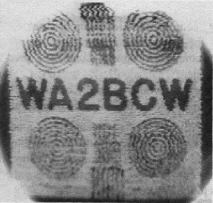
\includegraphics[width=0.7\linewidth]{figs/obrazek1.png}
	\caption{两个不同的图像使用 Martin M1 模式发射的SSTV频谱}
\end{figure}

\begin{figure}
	\centering
	\subfigure[50x38]{
		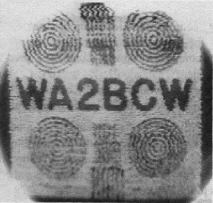
\includegraphics[width=0.45\linewidth]{figs/obrazek1.png}}
	\subfigure[120x90]{
		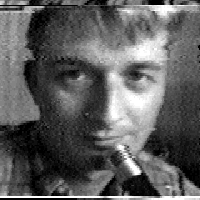
\includegraphics[width=0.45\linewidth]{figs/copthorn.png}}
	\caption{图像质量取决于分辨率}
\end{figure}


\section{图像分辨率}

分辨率是告诉人们能在一张图像里存储多少细节的一个功能,见图2.2。分辨率有两个参数:水平分辨率——图像的列数×图像的行数——垂直分辨率。

在电视科技中,垂直分辨率(行数)更加重要,它由SSTV模式的选择来定义。要获得水平分辨率更加复杂。

正如在前文中提到的,图像是通过短波SSB频道广播出去的,最大频宽是被限制的。

SSTV是一种模拟模式,它不能无损地传输图像。在接收端的图像并不是和发送端的图像完全一样。即使通信频道没有任何干扰或噪音,图像仍然会因为传输速度和有限的带宽而失真。传输速度越快,失真结果越大。因此很难说一个SSTV图像的水平分辨率是多少。

大多数模式都发送240行的图像,图像以4:3的宽高比在屏幕上显示。我们可以说列数是240×4/3=320。这个数值对应着理论上的分辨率,但不是真实的图像分辨率。

测试图(图2.3)被用于测试图像的水平分辨率。分辨率图像包含了从疏到密各种密度的黑白交叉条纹。这张图片和普通照片的对比在图2.1。

所有在图2.3中的模式都有320列。但我们可以看到,不是所有模式都能发送实际质量的图像。括号中的注释描述了发送1像素需要的大致时间。在Martin M2模式下我们很难分辨出第二细的网格,M1模式加倍了传输时间,它能没有问题地传输这个网格,但是最细的网格是失真的。与图2.4中的真实图像对比。列出的最后两种模式有更长的传输时间,能够发送最细致的细节。不幸的是,由于传输速度变慢,它很难得到补偿。

\begin{figure}
	\centering
	\subfigure[原始测试图案]{
		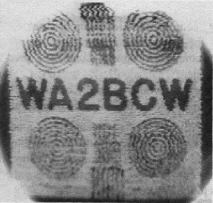
\includegraphics[width=0.45\linewidth]{figs/obrazek1.png}}
	\subfigure[Martin M2(~220μs)]{
		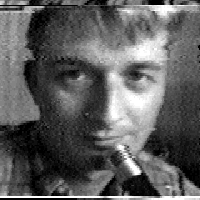
\includegraphics[width=0.45\linewidth]{figs/copthorn.png}}
	\subfigure[Robot 36 彩色]{
		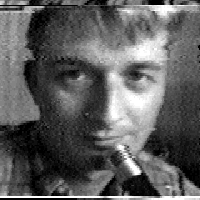
\includegraphics[width=0.45\linewidth]{figs/copthorn.png}}
	\subfigure[Martin M1]{
		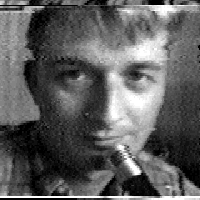
\includegraphics[width=0.45\linewidth]{figs/copthorn.png}}
	\subfigure[MP115]{
		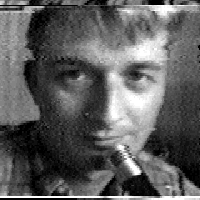
\includegraphics[width=0.45\linewidth]{figs/copthorn.png}}
	\subfigure[Scottie DX]{
		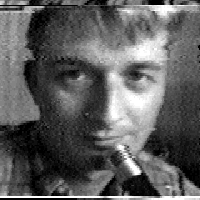
\includegraphics[width=0.45\linewidth]{figs/copthorn.png}}	
	\caption{几种SSTV模式水平分辨率的对比}
\end{figure}

\begin{figure}
	\centering
	\subfigure[Martin M1]{
		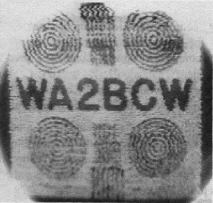
\includegraphics[width=0.45\linewidth]{figs/obrazek1.png}}
	\subfigure[Martin M2]{
		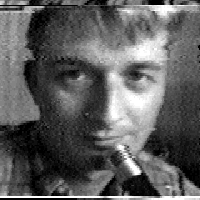
\includegraphics[width=0.45\linewidth]{figs/copthorn.png}}
	\caption{在14MHz现实环境下两种模式的对比}
\end{figure}


\section{行速度}

选择适合的SSTV模式时最重要的一个参数就是传输图像所需的总时间。

由于目前的传输速度,SSTV正变得和无线传真相似。因此,模式参数并不是由水平和垂直扫描率决定的,而是由一分钟传输的行数——行每分种(lpm)决定的。

行速度取决于选择的模式。范围从57 lpm(Scottie DX),用近5分钟的时间传输高质量的彩色图像(320×240),到1000 lpm,用8秒传输黑白图像(128×128)。SSTV模式和它们的特性会在下文讲述。

\section{黑白传输}

对于一个黑白单色图像的发送,仅需要一个信号。它表示每个图像元素的亮度Y。

从1500Hz(黑色)到2300Hz(白色)的频率范围被用来传输图像信息。在这个范围内的每个频率表示一个特定的亮度——灰色的等级。

人类视觉能分辨很大范围的亮度,但只能接受实际亮度的几何平均值。围绕这个值,大约100到110个灰度等级可以被分辨出来。

根据这个事实,一个理想的传输可以被认为是128个灰度等级。在这个数量级上,平均观察者通常不会看到相邻等级间的转换。

如果我们想要用128个灰度等级发送图像,信号等级的距离会是800Hz/128=6.25Hz。最低的频率是黑色,最高的频率是白色,其余的126个灰度在这两个频率之间线性排列。

一个传输更多灰度等级(例如256个等级)会带来的问题是对解调器需求的增加。解调器必须能够补偿发射机和接收机间的频率偏移。在这个例子中,两个亮度等级间的距离是3.125Hz,为了确保所有灰度等级的纯净发送,需要与通信路径上的干扰保持相对大的距离。

通常我们可以选择一个相对低的亮度分辨率,在这个分辨率下只能选择64个等级。这对解调器的要求更低,因为解调器只需要分辨12.5Hz的步进。

用灰度真实地再现彩色图像是另一个难题。人类视觉不能同时感知三种颜色分量的亮度。当我们观察相同亮度的三种光(红色、绿色和蓝色),我们的感知会觉得绿色光是最亮的,红色和蓝色并没有那么亮。

但是一个黑白电视摄相机只会扫描光强度等级,由此产生的图像会看起来像所有颜色都相同。它们会根据它们的强度以相同的灰度等级表示。由于这个事实,一个从基本颜色分量R、G和B(红、绿和黑)构成的有效的灰度图像Y被定义为:

$Y=0.30R+0.59G+0.11B$

请注意,最大的因数0.59只是绿色的,所以接近60\%我们看到的颜色取决于绿色分,只有40\%来自其余的颜色成分!这个公式是用于简化黑白图像使用的彩色扫描转换器。在过去,黑白图像并不是以真实的灰度图像发送的,亮度信号是从图像里绿色分量的亮度得来的。同一个图像的真实黑白图像和绿色分量的区别通常是微不足道的。

\begin{figure}
	\centering
	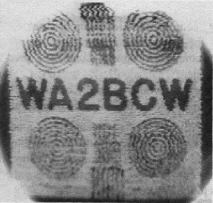
\includegraphics[width=0.7\linewidth]{figs/obrazek1.png}
	\caption{黑白图像的扫描行}
\end{figure}

\begin{figure}
	\centering
	\subfigure[红色分量]{
		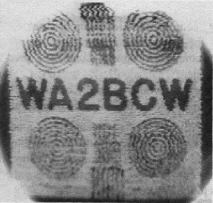
\includegraphics[width=0.3\linewidth]{figs/obrazek1.png}}
	\subfigure[绿色分量]{
		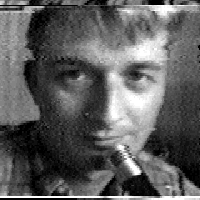
\includegraphics[width=0.3\linewidth]{figs/copthorn.png}}
	\subfigure[蓝色分量]{
		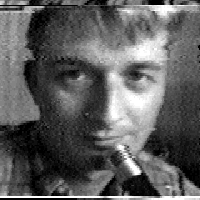
\includegraphics[width=0.3\linewidth]{figs/copthorn.png}}
	\subfigure[真实彩色图像]{
		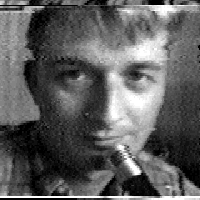
\includegraphics[width=0.3\linewidth]{figs/copthorn.png}}
	\subfigure[真实灰度]{
		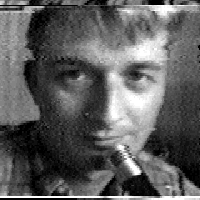
\includegraphics[width=0.3\linewidth]{figs/copthorn.png}}
	\subfigure[亮度]{
		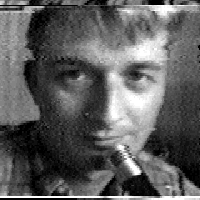
\includegraphics[width=0.3\linewidth]{figs/copthorn.png}}	
	\caption{彩色图像到基本颜色分量的分解}
\end{figure}


\section{彩色传输}

\subsection{加色法模型}

每种颜色都能被分解成三种基本色——红色、绿色和蓝色。加色法模型通过结合这三种基本色来产生其他颜色。

在图像传输过程中,图像在发射端被分解成这三种互相独立的颜色分量,然后将它们逐渐发射出去,再在接收端重新结合成一幅图像。

如果在800Hz的图像频道内可以检测到64个频率等级,那么每个颜色分量就包含64种亮度等级。所得到的彩色图像就包含64×6464=256144种颜色。如果解调器能分辨256个等级,那就有可能传送超过160万=$256^{3}$种颜色。彩色SSTV传输可以满足对色彩深度最苛刻的要求。

一些彩色SSTV系统也利用了人类视觉的一种属性,就是对基本颜色分量的不同敏感度。在这个例子中,图像的扫描行并没有给每个颜色分量分解成三等份。因为人眼对绿色最敏感,每行的最大部分作为绿色,其余部分作为红色和蓝色。例如G:R:B的比例4:2:2。

加色法模型需要更长的时间去传输,但是它提供了真实的色彩。

\begin{figure}
	\centering
	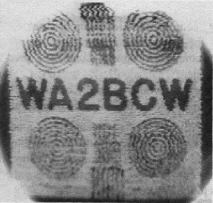
\includegraphics[width=0.7\linewidth]{figs/obrazek1.png}
	\caption{彩色图像到RGB信号的分解图}
\end{figure}


\subsection{复合颜色模型}

第二种彩色传输类型叫做YCrCb。事实上这是一种和彩色快扫描电视类似的系统,每个颜色分量R、G和B,被转化成亮度和色度(颜色信息)信号。和RGB不同,这种传输的时间更短。这种颜色编码被用在电视广播中,黑白和彩色的兼容性上,黑白电视也可以接收彩色广播。

\begin{figure}
	\centering
	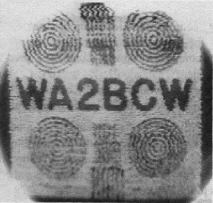
\includegraphics[width=0.7\linewidth]{figs/obrazek1.png}
	\caption{彩色图像到YCrCb信号的分解图}
\end{figure}

图像扫描行包含了颜色的两种分量——亮度和色度。色度信号是由两种不同的颜色信号R-Y和B-Y组成的。Y信号被称作亮度,它包含了对应公式Y=0.30R+0.59G+0.10B的亮度信号。Y是从红色和蓝色减去的色度信号。

在接收端,单独的颜色分量被复原:R=(R-Y)+Y,B=(B-Y)+Y。

我们还需要绿色分量G,它是从R-Y和B-Y推导出的,用公式G=Y-0.51(R-Y)-0.19(B-Y)。至此我们得到了复合颜色模型。

在SSTV中有两种YCrCb彩色传输格式被使用。第一种格式是4:2:2,两种色度信号在同一行传输(于Y信号相比时间减少一半)。第二种格式是4:2:0,只包含一种色度信号。比如奇数扫描行只包含R-Y,偶数扫描行只包含B-Y。然后通过原始图像的两个连续扫描行的平均值得到色度信号。

这种传输格式与RGB相比的优点是显著缩短的传输时间。与RGB相比,YCrCb大约只需要一半时间,而且保证几乎相同的图像质量。

与RGB模型相比,它的缺点是图像信息的丢失,在使用4:2:0格式的时候更加明显。另外,它需要精确的收发信机调谐,否则色彩信息会失真,这也是为什么YCRCB编码更少的被使用的原因。根据载波的正向或负向偏移,图像的色调会强烈地偏向粉色或绿色,见图3.9。

\begin{figure}
	\centering
	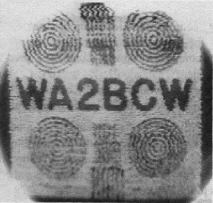
\includegraphics[width=0.7\linewidth]{figs/obrazek1.png}
	\caption{当电台调整不当时YCrCb的颜色失真}
\end{figure}

彩色FSTV传输在使用YCrCb的同时也使用特殊的方法和调制(在PAL、SECAM中)来消除这种可能发生在传输路径上的颜色失真。不幸的是,这个功能并不存在于SSTV,所以选择性衰减会导致图像的彩色重影。

使用YCrCb传输的SSTV系统的抗干扰性比对应的RGB模式更低,见图3.10。

当发射机载波有明显的±200Hz偏移时,RGB模型会因为低对比度或增加的亮度而失真,从而提供比YCrCb更好的色彩。

\begin{figure}
	\centering
	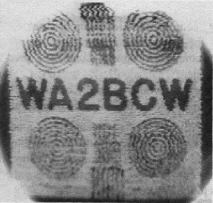
\includegraphics[width=0.7\linewidth]{figs/obrazek1.png}
	\caption{当电台调整不当时RGB的颜色失真}
\end{figure}


\section{同步}

\subsection{水平同步}

\subsection{垂直同步-VIS码}
垂直间隔信号

\subsection{附加同步数据}